% Supplementary Information (input by supplement.tex). Numbering follows the journal's style:
% "Supplementary Table 1", "Supplementary Fig. 1", "Supplementary Section 1".
\makeatletter
\def\thetable{\arabic{table}}
\def\theHtable{S\arabic{table}}
\def\tablename{Supplementary Table}
\def\thefigure{\arabic{figure}}
\def\theHfigure{S\arabic{figure}}
\def\figurename{Supplementary Fig.}
\def\thesection{\arabic{section}}
\def\theHsection{S\arabic{section}}
\def\SI@prefix@section{Supplementary Section~}
\def\@seccntformat#1{\csname SI@prefix@#1\endcsname\csname the#1\endcsname\quad}
\setlength{\@fptop}{0pt}  % a page of floats starts at the top, not vertically centred
\setlength{\@fpbot}{0pt plus 1fil}
\setlength{\@fpsep}{\floatsep}  % and its floats are stacked, not spread over the page
\makeatother
\setcounter{table}{0}
\setcounter{figure}{0}
\setcounter{section}{0}

\noindent\textbf{Contents}
{\setstretch{1.1}  % compact, so that Supplementary Table 1 fits below
\begin{itemize}\setlength{\itemsep}{0pt}
  \item Supplementary Table~\ref{tab:characteristics}: characteristics of the benchmark splits
  \item Supplementary Table~\ref{tab:provenance}: stated measurements and labelled values in the printed code output
    (post hoc)
  \item Supplementary Table~\ref{tab:perclass}: discrimination by superclass on the test fold
  \item Supplementary Table~\ref{tab:benchmark}: macro AUROC compared with published results
  \item Supplementary Table~\ref{tab:statements}: discrimination by diagnostic statement (post hoc)
  \item Supplementary Table~\ref{tab:measurements}: measurements stated in the key findings (post hoc)
  \item Supplementary Table~\ref{tab:subgroups}: macro AUROC by subgroup (post hoc)
  \item Supplementary Fig.~\ref{fig:usage}: code runs, output tokens and cost per record
  \item Supplementary Fig.~\ref{fig:curves}: ROC and precision--recall curves; reliability curves (post hoc)
  \item Supplementary Section~\ref{app:example}: example user message
  \item Supplementary Section~\ref{app:transcript}: transcript of the example record
  \item Supplementary Section~\ref{app:prompt}: system prompt
  \item Supplementary Section~\ref{app:schema}: output schema
\end{itemize}
\par}
% Items are numbered, and placed, in the order of their first citation in the manuscript (tables, figures and
% sections each in their own sequence); \FloatBarrier keeps the figures from floating ahead of the tables.

\CharacteristicsTable
\ProvenanceTable

\begin{table}[!htbp]
  \centering
  \caption{\textbf{Discrimination by superclass on the test fold} (\NTest{} records). The model and the age-and-sex
  control, with 95\% percentile bootstrap CIs from the \NBoot{} resamples of the primary analysis; of the values by
  class, only the model's AUROC, without its CI, was pre-specified. Positives: test records with the superclass label,
  $n$ (\%). Difference: model minus control, paired on the same resamples. AUPRC: average precision of the model;
  without skill, it equals the class prevalence (for the macro average, the mean prevalence).}
  \label{tab:perclass}
  \footnotesize\setlength{\tabcolsep}{5pt}
  \begin{tabular}{lrcccc}
    \toprule
    Class & Positives, $n$ (\%) & AUROC [95\% CI] & Control AUROC & Difference [95\% CI] & AUPRC \\
    \midrule
    NORM & \PosNORM{} (\PrevNORM) & \MainNORM{} [\MainNORMLow, \MainNORMHigh] & \AgeSexNORM &
      $\CodeVsAgeSexNORM$ [$\CodeVsAgeSexNORMLow$, $\CodeVsAgeSexNORMHigh$] & \AUPRCNORM \\
    MI & \PosMI{} (\PrevMI) & \MainMI{} [\MainMILow, \MainMIHigh] & \AgeSexMI &
      $\CodeVsAgeSexMI$ [$\CodeVsAgeSexMILow$, $\CodeVsAgeSexMIHigh$] & \AUPRCMI \\
    STTC & \PosSTTC{} (\PrevSTTC) & \MainSTTC{} [\MainSTTCLow, \MainSTTCHigh] & \AgeSexSTTC &
      $\CodeVsAgeSexSTTC$ [$\CodeVsAgeSexSTTCLow$, $\CodeVsAgeSexSTTCHigh$] & \AUPRCSTTC \\
    CD & \PosCD{} (\PrevCD) & \MainCD{} [\MainCDLow, \MainCDHigh] & \AgeSexCD &
      $\CodeVsAgeSexCD$ [$\CodeVsAgeSexCDLow$, $\CodeVsAgeSexCDHigh$] & \AUPRCCD \\
    HYP & \PosHYP{} (\PrevHYP) & \MainHYP{} [\MainHYPLow, \MainHYPHigh] & \AgeSexHYP &
      $\CodeVsAgeSexHYP$ [$\CodeVsAgeSexHYPLow$, $\CodeVsAgeSexHYPHigh$] & \AUPRCHYP \\
    \midrule
    Macro average & -- & \MainAUROC{} [\MainAUROCLow, \MainAUROCHigh] & \AgeSexAUROC &
      $\CodeVsAgeSex$ [$\CodeVsAgeSexLow$, $\CodeVsAgeSexHigh$] & \MainAUPRC \\
    \bottomrule
  \end{tabular}
\end{table}

\begin{table}[!htbp]
  \centering
  \caption{\textbf{Macro AUROC on the PTB-XL diagnostic superclass task (5 superclasses).} Published values as reported by
  their authors; this work on all \NTest{} test-fold records with 95\% percentile bootstrap CIs in brackets (\NBoot{}
  resamples; results by class in Supplementary Table~\ref{tab:perclass}).}
  \label{tab:benchmark}
  \footnotesize\renewcommand{\arraystretch}{0.97}
  % Generated by python analysis/si.py from benchmarks/ptbxl_superdiagnostic_published.csv
\begin{tabular}{L{0.52\linewidth}L{0.19\linewidth}l}
\toprule
Method & Input & Macro AUROC \\
\midrule
\multicolumn{3}{l}{\emph{Original PTB-XL benchmark: supervised, trained on folds 1--8}} \\
  \quad ensemble of the benchmark models~\citep{Strodthoff2021} & signal (100 Hz) & 0.934 (05) \\
  \quad resnet1d\_wang~\citep{Strodthoff2021} & signal (100 Hz) & 0.930 (05) \\
  \quad xresnet1d101~\citep{Strodthoff2021} & signal (100 Hz) & 0.928 (05) \\
  \quad lstm~\citep{Strodthoff2021} & signal (100 Hz) & 0.927 (05) \\
  \quad fcn\_wang~\citep{Strodthoff2021} & signal (100 Hz) & 0.925 (06) \\
  \quad inception1d~\citep{Strodthoff2021} & signal (100 Hz) & 0.921 (06) \\
  \quad Wavelet+NN~\citep{Strodthoff2021} & wavelet features & 0.874 (07) \\
\midrule
\multicolumn{3}{l}{\emph{Later supervised models}} \\
  \quad RecursiveECG (LLM-refined classifier)~\citep{deng2026recursiveecg}$^\dagger$ & signal (100 Hz) & 0.937 \\
  \quad MS-SSM (S6)~\citep{karami2025msssm}$^\dagger$ & signal (100 Hz) & 0.935 \\
  \quad MultiresNet~\citep{shi2023multires} & signal (100 Hz) & 0.934 \\
  \quad S4~\citep{almasud2026benchmarking}$^\dagger$ & signal (100 Hz) & 0.932 \\
  \quad Chimera~\citep{behrouz2024chimera}$^\dagger$ & signal (100 Hz) & 0.930 \\
  \quad SpaceTime~\citep{zhang2023spacetime}$^\dagger$ & signal (100 Hz) & 0.929 \\
\midrule
\multicolumn{3}{l}{\emph{Pretrained on large ECG corpora, then fine-tuned on PTB-XL}} \\
  \quad HuBERT++ (S4 backbone)~\citep{almasud2026pretraining}$^\dagger$ & signal (240 Hz) & 0.936 \\
  \quad ECGFounder~\citep{almasud2026benchmarking}$^\dagger$ & signal & 0.935 \\
  \quad ECG-CPC~\citep{almasud2026benchmarking}$^\dagger$ & signal (240 Hz) & 0.934 \\
  \quad ECG-JEPA~\citep{kim2024ecgjepa} & signal (250 Hz) & 0.931 \\
  \quad xECG~\citep{lunelli2025benchecg} & signal (100 Hz) & 0.928 \\
  \quad HuBERT-ECG (base)~\citep{coppola2024hubertecg} & signal (100 Hz) & 0.911 \\
\midrule
\multicolumn{3}{l}{\emph{Zero-shot ECG--language models (encoder pretrained on ECGs with reports or report-derived labels)}} \\
  \quad SuPreME~\citep{cai2025supreme} & signal & 0.782 \\
  \quad MELP~\citep{wang2025melp} & signal & 0.762 \\
  \quad D-BETA~\citep{pham2025dbeta} & signal & 0.762 \\
  \quad MERL~\citep{liu2024merl} & signal & 0.742 \\
\midrule
\multicolumn{3}{l}{\emph{Multimodal LLMs instruction-tuned on ECG data}} \\
  \quad GEM~\citep{lan2025gem}$^\dagger$ & signal + image & 0.834 \\
  \quad PULSE~\citep{liu2024teach}$^\dagger$ & image & 0.829 \\
\midrule
\multicolumn{3}{l}{\emph{General-purpose multimodal LLMs, zero-shot, ECG images}} \\
  \quad GPT-4o~\citep{liu2024teach}$^\dagger$ & image & 0.556 \\
  \quad Claude 3.5 Sonnet~\citep{liu2024teach}$^\dagger$ & image & 0.540 \\
  \quad Gemini 1.5 Pro~\citep{liu2024teach}$^\dagger$ & image & 0.507 \\
\midrule
\multicolumn{3}{l}{\emph{This work (test fold, \NTest{} records)}} \\
  \quad General-purpose LLM with a Python sandbox\newline\hspace*{1em}(\ModelID) & raw signal (500 Hz), age, sex & \MainAUROC{} [\MainAUROCLow, \MainAUROCHigh] \\
  \quad Age and sex only (control, logistic regression) & demographics & \AgeSexAUROC{} [\AgeSexAUROCLow, \AgeSexAUROCHigh] \\
\bottomrule
\end{tabular}

  \par\smallskip
  \begin{minipage}{\linewidth}\scriptsize
  Original benchmark: uncertainty as printed in~\citet{Strodthoff2021} (bootstrap, last digits); these models were
  evaluated on the PTB-XL release before version 1.0.2, whose test fold had 2{,}163 records with a superclass; the
  \NTest{} test records used here (version 1.0.3) are a subset of them with identical superclass labels.
  $^\dagger$Split not stated, or a different test set (the multimodal-LLM rows use a \NOtherTestSet-record hold-out set;
  RecursiveECG uses all 2{,}203 fold-10 records of an earlier PTB-XL release, including records without a
  superclass); not directly comparable. RecursiveECG: a supervised classifier, initially a 12-lead ResNet, whose
  architecture and code an LLM agent (DeepSeek-V4-Pro) revised in up to five rounds, keeping revisions that improved
  validation performance; mean of 5 runs, each repeating the design process. HuBERT-ECG's self-supervised pretraining
  corpus includes PTB-XL (unlabelled). PULSE and general-purpose LLM values: ref.~\citenum{liu2024teach}, Table~1.
  SuPreME was pretrained on diagnostic labels extracted from reports by a language model, not on the report text.
  Inputs differ: only this work received age and sex, and it received the signal at 500\,Hz (other sampling rates as
  listed). Comparisons with published results are informal (no per-record predictions available).
  \end{minipage}
\end{table}

\StatementTable
\MeasurementTable
\SubgroupTable
\FloatBarrier

\begin{figure}[!htbp]
  \centering
  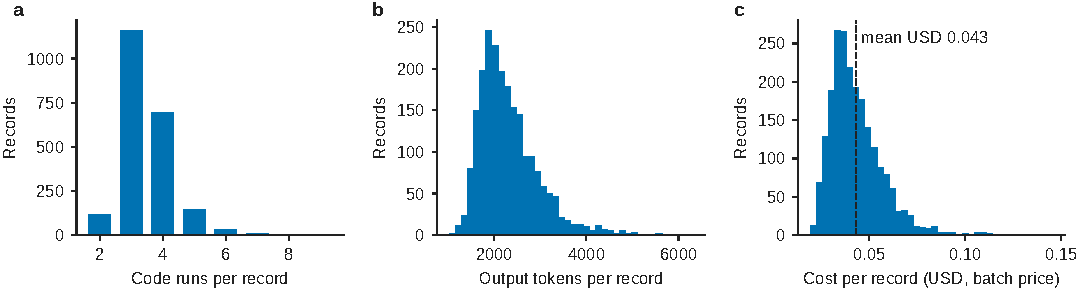
\includegraphics[width=\linewidth]{figS2_usage}
  \caption{\textbf{Tool use and cost per record in the test run} (\NTest{} records). \textbf{a}, Number of code runs.
  \textbf{b}, Output tokens (reasoning, code and answer). \textbf{c}, Cost at batch prices; the dashed line is the
  mean. Input tokens, not shown, averaged \InputTokensMean{} per record (\CacheReadPct\% read from the prompt cache);
  cache writes accounted for \CacheWriteCostPct\% of the cost.}
  \label{fig:usage}
\end{figure}

\begin{figure}[!htbp]
  \centering
  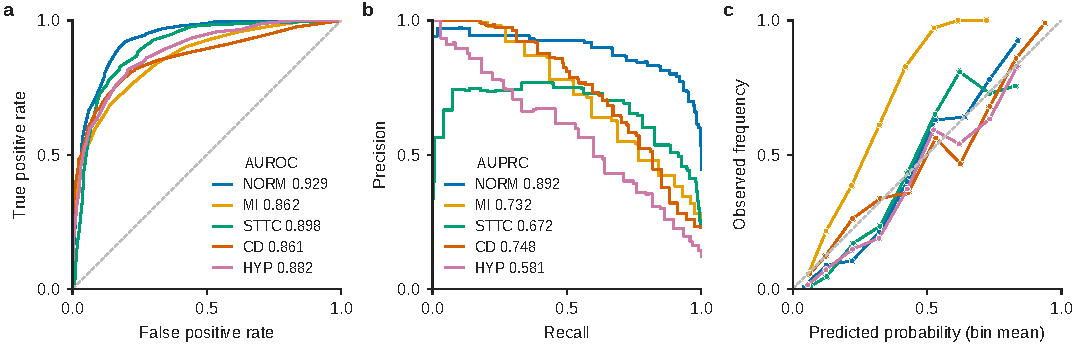
\includegraphics[width=\linewidth]{figS1_curves}
  \caption{\textbf{ROC, precision--recall and reliability curves on the test fold.} \textbf{a}, ROC;
  \textbf{b}, precision--recall (without skill, precision equals the class prevalence); \textbf{c}, reliability (post
  hoc; colours as in \textbf{a} and \textbf{b}); all \NTest{} records. Reliability: predicted probabilities in ten
  equal-width bins (a probability on a bin edge goes to the upper bin, as for the expected calibration error; bins with
  at least 20 records shown), mean predicted probability against observed frequency; the dashed line is perfect
  calibration.}
  \label{fig:curves}
\end{figure}
\clearpage

\section{Example user message}\label{app:example}
The user message of the record in Fig.~\ref{fig:example} (PTB-XL \texttt{ecg\_id} \ExampleECGID, validation fold), as
sent (the long line is wrapped for the page, with the continuation indented), and the first rows of the attached file.
\begin{footnotesize}
\begin{verbatim}
User message (text block):
Record d0043. The attached file d0043.csv holds the raw 10-second 12-lead recording. Patient: age 
  25 years, male. Classify it as described, then answer with the JSON object only.

Attached file (container_upload block): d0043.csv, 5,000 data rows. First rows:
t_ms,I,II,III,aVR,aVL,aVF,V1,V2,V3,V4,V5,V6
0,-0.065,0.265,0.330,-0.100,-0.198,0.297,0.050,-0.215,-0.085,-0.130,-0.220,-0.155
2,-0.065,0.265,0.330,-0.100,-0.198,0.297,0.050,-0.215,-0.085,-0.130,-0.220,-0.155
4,-0.065,0.265,0.330,-0.100,-0.198,0.297,0.050,-0.215,-0.085,-0.130,-0.220,-0.155
...
(The first 6 samples are identical, as in the PTB-XL source file.)
\end{verbatim}
\end{footnotesize}


\section{Transcript of the example record}\label{app:transcript}
Every code run of the model for the record in Fig.~\ref{fig:example}, with the printed output (long outputs cut after
30 lines, as marked), the summarized reasoning returned by the API and the final answer. Lines longer than the page
are wrapped; non-ASCII symbols are transliterated.
% Generated from dev200b_v2/results.jsonl, record d0043 (PTB-XL ecg_id 30)
\begin{scriptsize}
\begin{verbatim}
=== Code run 1: command ===
cd $INPUT_DIR; head -3 d0043.csv; wc -l d0043.csv
=== Code run 1: printed output ===
t_ms,I,II,III,aVR,aVL,aVF,V1,V2,V3,V4,V5,V6
0,-0.065,0.265,0.330,-0.100,-0.198,0.297,0.050,-0.215,-0.085,-0.130,-0.220,-0.155
2,-0.065,0.265,0.330,-0.100,-0.198,0.297,0.050,-0.215,-0.085,-0.130,-0.220,-0.155
5001 d0043.csv

=== Code run 2: command ===
cd $INPUT_DIR; cat > /tmp/a.py <<'EOF'
import pandas as pd,numpy as np
from scipy.signal import butter,filtfilt,find_peaks
d=pd.read_csv('d0043.csv');fs=500
L=list(d.columns[1:]);X=d[L].values
b,a=butter(2,[0.5,40],btype='band',fs=fs);Y=filtfilt(b,a,X,axis=0)
e=np.sum(np.abs(np.diff(Y,axis=0)),axis=1)
pk,_=find_peaks(e,height=np.percentile(e,98)*0.4,distance=int(0.3*fs))
# refine on lead II abs
rr=np.diff(pk)/fs
print('HR',60/rr.mean(),'RR sd',rr.std(),len(pk))
print(np.round(rr,3))
beats=np.array([Y[p-300:p+400] for p in pk if p>300 and p+400<len(Y)])
M=np.median(beats,axis=0)
t=np.arange(-300,400)*2
for i,l in enumerate(L):
  m=M[:,i]
  print(l,' '.join(f'{v:.2f}' for v in m[250:450:5]))
np.save('/tmp/M.npy',M)
EOF
python /tmp/a.py
=== Code run 2: printed output ===
HR 63.81620931716655 RR sd 0.009816312953446382 11
[0.932 0.944 0.936 0.928 0.946 0.954 0.958 0.942 0.93  0.932]
I -0.07 -0.07 -0.07 -0.08 -0.10 -0.09 0.07 0.33 0.62 0.74 0.38 -0.18 -0.32 -0.25 -0.16 -0.09 -0.08 -0.06 
  -0.04 -0.04 -0.03 -0.03 -0.01 -0.00 0.01 0.03 0.05 0.07 0.09 0.12 0.14 0.17 0.21 0.24 0.26 0.26 0.25 
  0.22 0.18 0.14
II -0.07 -0.09 -0.08 -0.09 -0.10 -0.07 0.13 0.47 0.81 0.91 0.30 -0.26 -0.51 -0.43 -0.26 -0.15 -0.09 
  -0.07 -0.06 -0.05 -0.03 -0.03 -0.02 -0.01 0.00 0.02 0.04 0.06 0.08 0.09 0.12 0.14 0.17 0.20 0.21 0.22 
  0.21 0.20 0.17 0.13
III -0.01 -0.01 -0.01 -0.00 -0.00 0.02 0.05 0.12 0.18 0.18 -0.01 -0.09 -0.20 -0.18 -0.10 -0.04 -0.01 
  -0.01 -0.00 -0.01 0.00 0.01 -0.01 -0.01 -0.02 -0.02 -0.02 -0.02 -0.01 -0.03 -0.02 -0.03 -0.04 -0.05 
  -0.06 -0.06 -0.04 -0.03 -0.01 -0.00
aVR 0.08 0.08 0.08 0.09 0.10 0.08 -0.09 -0.40 -0.71 -0.83 -0.35 0.24 0.42 0.34 0.21 0.12 0.09 0.06 0.05 
  0.04 0.03 0.03 0.02 0.01 -0.00 -0.02 -0.05 -0.06 -0.08 -0.10 -0.13 -0.16 -0.19 -0.21 -0.23 -0.23 -0.22 
  -0.21 -0.17 -0.13
aVL -0.04 -0.03 -0.03 -0.04 -0.05 -0.06 0.01 0.10 0.23 0.28 0.20 -0.06 -0.06 -0.04 -0.03 -0.03 -0.04 
  -0.03 -0.02 -0.01 -0.01 -0.01 -0.00 0.01 0.01 0.02 0.03 0.05 0.05 0.07 0.08 0.10 0.12 0.15 0.16 0.16 
  0.15 0.12 0.10 0.07
aVF -0.04 -0.05 -0.05 -0.05 -0.05 -0.03 0.09 0.30 0.49 0.53 0.14 -0.17 -0.35 -0.30 -0.18 -0.09 -0.05 
  -0.04 -0.03 -0.03 -0.02 -0.01 -0.01 -0.01 -0.00 0.00 0.02 0.02 0.03 0.03 0.05 0.06 0.06 0.08 0.08 0.09 
  0.08 0.08 0.09 0.07
V1 0.04 0.04 0.04 0.06 0.13 0.18 0.05 -0.34 -0.88 -1.25 -1.01 -0.46 -0.23 -0.15 -0.01 0.06 0.09 0.10 
  0.10 0.10 0.10 0.09 0.09 0.09 0.08 0.08 0.07 0.07 0.06 0.05 0.04 0.02 0.00 -0.01 -0.03 -0.04 -0.03 
  -0.03 -0.02 -0.01
V2 -0.02 -0.02 -0.03 -0.01 0.16 0.34 0.24 -0.84 -2.44 -3.10 -2.61 -1.68 -1.12 -0.73 -0.26 0.02 0.12 0.17 
  0.19 0.21 0.23 0.25 0.28 0.30 0.33 0.36 0.39 0.44 0.50 0.57 0.63 0.69 0.75 0.78 0.78 0.77 0.73 0.64 
  0.55 0.45
V3 -0.08 -0.07 -0.08 -0.06 0.03 0.18 0.31 -0.10 -1.09 -1.63 -1.70 -1.44 -1.08 -0.67 -0.25 -0.02 0.07 
  0.11 0.14 0.16 0.18 0.20 0.23 0.26 0.29 0.32 0.36 0.41 0.46 0.53 0.59 0.64 0.69 0.72 0.70 0.67 0.60 
  0.51 0.42 0.33
V4 -0.13 -0.13 -0.12 -0.12 -0.12 -0.03 0.21 0.58 1.03 1.26 0.39 -0.70 -0.82 -0.56 -0.30 -0.15 -0.09 
  -0.06 -0.04 -0.02 -0.00 0.02 0.04 0.06 0.08 0.10 0.13 0.17 0.20 0.24 0.29 0.34 0.37 0.39 0.38 0.38 
  0.35 0.32 0.26 0.20
V5 -0.13 -0.13 -0.12 -0.12 -0.17 -0.16 0.05 0.67 1.68 2.19 0.96 -0.36 -0.56 -0.43 -0.28 -0.19 -0.15 
  -0.12 -0.10 -0.10 -0.09 -0.07 -0.05 -0.04 -0.03 -0.01 0.01 0.03 0.06 0.09 0.12 0.16 0.19 0.22 0.25 
  0.26 0.26 0.24 0.20 0.15
V6 -0.10 -0.10 -0.10 -0.10 -0.15 -0.17 -0.01 0.48 1.32 1.75 0.97 -0.05 -0.33 -0.28 -0.21 -0.15 -0.12 
  -0.11 -0.10 -0.09 -0.08 -0.07 -0.06 -0.05 -0.04 -0.03 -0.02 0.00 0.02 0.04 0.06 0.09 0.12 0.15 0.17 
  0.19 0.20 0.19 0.16 0.12

=== Code run 3: command ===
cd /tmp; cat > b.py <<'EOF'
import numpy as np
M=np.load('/tmp/M.npy');L='I II III aVR aVL aVF V1 V2 V3 V4 V5 V6'.split()
for l in ['II','V1','V2','V5']:
  i=L.index(l);print(l,' '.join(f'{v:.2f}' for v in M[150:300:4,i]))
g=np.sum(np.abs(np.gradient(M,axis=0)),axis=1)
print(' '.join(f'{v:.2f}' for v in g[240:360:3]))
EOF
python b.py
=== Code run 3: printed output ===
II -0.07 -0.07 -0.06 -0.06 -0.06 -0.07 -0.06 -0.06 -0.05 -0.05 -0.03 -0.01 0.01 0.03 0.04 0.05 0.05 0.04 
  0.04 0.02 -0.00 -0.03 -0.05 -0.07 -0.07 -0.07 -0.09 -0.09 -0.09 -0.09 -0.10 -0.09 0.02 0.25 0.54 0.81 
  0.94 0.59
V1 0.05 0.04 0.04 0.05 0.04 0.04 0.05 0.06 0.06 0.07 0.07 0.08 0.09 0.08 0.07 0.05 0.04 0.03 0.03 0.04 
  0.04 0.04 0.04 0.04 0.04 0.04 0.04 0.04 0.04 0.07 0.13 0.18 0.14 -0.07 -0.44 -0.88 -1.21 -1.19
V2 -0.02 -0.02 -0.02 -0.02 -0.02 -0.02 -0.02 -0.02 -0.01 -0.00 0.00 0.01 0.02 0.02 0.02 0.00 -0.03 -0.04 
  -0.04 -0.03 -0.03 -0.03 -0.03 -0.03 -0.03 -0.02 -0.02 -0.02 -0.03 0.01 0.16 0.31 0.35 -0.06 -1.16 
  -2.44 -3.07 -2.90
V5 -0.11 -0.11 -0.11 -0.11 -0.11 -0.11 -0.11 -0.10 -0.10 -0.09 -0.08 -0.08 -0.07 -0.07 -0.07 -0.07 -0.07 
  -0.07 -0.07 -0.07 -0.08 -0.09 -0.10 -0.11 -0.12 -0.13 -0.13 -0.12 -0.12 -0.13 -0.17 -0.17 -0.07 0.24 
  0.85 1.68 2.23 1.62
0.02 0.02 0.02 0.02 0.01 0.01 0.01 0.01 0.04 0.10 0.13 0.13 0.23 0.49 0.88 1.22 1.40 1.11 0.29 1.09 1.70 
  1.47 0.78 0.33 0.30 0.42 0.43 0.33 0.20 0.12 0.07 0.06 0.04 0.04 0.03 0.02 0.03 0.02 0.03 0.03

=== Code run 4: command ===
cd /tmp; cat > c.py <<'EOF'
import numpy as np
M=np.load('/tmp/M.npy');L='I II III aVR aVL aVF V1 V2 V3 V4 V5 V6'.split()
bl=M[250:262].mean(0);M=M-bl
g=np.sqrt(np.sum(np.gradient(M,axis=0)**2,axis=1))
thr=0.1*g[260:340].max()
idx=np.where(g[200:360]>thr)[0]+200
print('on',idx.min(),'off',idx.max(),'QRS ms',(idx.max()-idx.min())*2)
on=idx.min();off=idx.max()
# T end: lead V2 
for l in L:
  i=L.index(l);m=M[:,i];q=m[on:on+25].min();
  print(f"{l:4s} R {m[on:off].max():.2f} S {m[on:off].min():.2f} J {m[off]:.2f} J60 {m[off+30]:.2f} T 
  {m[off+50:off+220][np.argmax(abs(m[off+50:off+220]))]:.2f}")
v=M[:,L.index('V2')];tp=off+50+np.argmax(v[off+50:off+250]);
d=np.gradient(v);k=tp+np.argmin(d[tp:tp+100]);te=k+int(v[k]/(-d[k]))
print('QT',(te-on)*2,'QTc',(te-on)*2/np.sqrt(0.94))
I=M[on:off,0].sum();F=M[on:off,5].sum();print('axis',np.degrees(np.arctan2(F*2/np.sqrt(3),I)))
EOF
python c.py
=== Code run 4: printed output ===
on 275 off 324 QRS ms 98
I    R 0.83 S -0.25 J -0.02 J60 0.04 T 0.34
II   R 1.03 S -0.43 J -0.08 J60 0.06 T 0.30
III  R 0.22 S -0.20 J -0.04 J60 0.02 T -0.05
aVR  R 0.34 S -0.93 J 0.06 J60 -0.05 T -0.31
aVL  R 0.31 S -0.04 J 0.01 J60 0.02 T 0.20
aVF  R 0.63 S -0.31 J -0.06 J60 0.03 T 0.13
V1   R 0.14 S -1.30 J 0.02 J60 0.05 T -0.08
V2   R 0.39 S -3.08 J 0.00 J60 0.27 T 0.81
V3   R 0.38 S -1.65 J 0.02 J60 0.28 T 0.79
V4   R 1.41 S -0.73 J -0.05 J60 0.14 T 0.52
V5   R 2.35 S -0.45 J -0.08 J60 0.05 T 0.38
V6   R 1.85 S -0.24 J -0.06 J60 0.02 T 0.30
QT 382 QTc 394.0029160708591
axis 30.67115572484157

=== Summarized thinking (as returned by the API; the full thinking is not returned) ===
I'm working out the baseline correction and amplitude measurements to calculate the Sokolow-Lyon index, 
  combining S wave depth in V1/V2 with R wave height in V5 to check for voltage criteria suggestive of 
  left ventricular hypertrophy.

Elevated voltage like this isn't unusual in a young man, so I'm also checking QRS duration by finding 
  onset and offset points, which comes out to roughly 100ms, before moving on to look at the P wave and 
  PR interval.
I'm measuring the P wave, PR interval, and QRS duration from the index positions, estimating PR around 
  150ms and QRS near 120ms. I'm also checking lead morphology across V1, V5/V6, and lead I for terminal 
  S waves, weighing whether this points toward a conduction pattern like RBBB despite no R' in V1.

I'm noticing terminal S waves across leads I, II, III, and slurring in V6, consistent with an S1S2S3 
  pattern that could just be a normal variant. I want to nail down QRS onset more precisely by checking 
  where V1/V2 deviate from baseline, then move on to computing ST segment and QT interval.
The axis looks like it's around +30-60 degrees with QRS duration roughly 98-110ms. The Sokolow-Lyon 
  voltage sums (3.65mV and 5.4mV) suggest voltage criteria for LVH, which is common in young males and 
  often gets labeled as LVH in datasets like PTB-XL even without other supporting findings; otherwise 
  everything else looks normal, though P wave amplitude is a bit low.

=== Final answer ===
{
 "records": [
  {
   "record_id": "d0043",
   "key_findings": "The rhythm is regular sinus at about 64 bpm, with PR about 150 ms, QRS about 100 ms, 
  QTc about 395 ms, a normal axis near +45 deg and no pathological Q waves or ST-T abnormality. High 
  precordial voltage (Sokolow-Lyon 3.65 mV = S V1 1.30 + R V5 2.35; S V2 3.1 mV) without strain is 
  voltage-only LVH, which can be a normal finding in a 25-year-old man.",
   "p_NORM": 0.5,
   "p_MI": 0.04,
   "p_STTC": 0.07,
   "p_CD": 0.1,
   "p_HYP": 0.42
  }
 ]
}
\end{verbatim}
\end{scriptsize}


\section{System prompt}\label{app:prompt}
The complete system prompt of the frozen configuration, identical for every request. The exact text is the file
\nolinkurl{prompts/reader_code_v2_measure.md} in the repository, whose SHA-256 hash begins \PromptSHA; here, long lines are wrapped for the page, with continuation lines indented.
% Generated from prompts/reader_code_v2_measure.md (sha256 c006aa662f4803fd126aad3dca504fd0e2a50702fc90cae717abf7381c075bde)
\begin{small}
\begin{verbatim}
You are an expert cardiologist with a Python sandbox. You will classify one 12-lead ECG 
  from its raw digital recording.

DATA
The message gives the patient's age and sex and attaches one CSV file (its name is the 
  record id, e.g. `d0001.csv`), available in the sandbox. Columns: `t_ms` (time in 
  milliseconds) and the 12 leads `I, II, III, aVR, aVL, aVF, V1, V2, V3, V4, V5, V6`, in 
  millivolts. Each row is one sample; the recording is 10 seconds long. The signal is 
  raw: it may contain baseline wander, noise or artefacts.

HOW TO WORK
Use Python (numpy, scipy and pandas are available; there is no internet access). Work in 
  two steps.

Step 1, measure. Filter the signal (baseline wander, mains noise), detect the beats, 
  align them and form a median beat per lead, and set the baseline from the PR segment. 
  Then compute and print this complete measurement table before judging anything:
- rhythm: heart rate, RR regularity, a P wave before each QRS (yes/no), extra or dropped 
  beats;
- intervals: PR, QRS duration (from the earliest onset to the latest offset over all 
  leads), QT and QTc (Bazett);
- frontal QRS axis;
- per lead: Q wave duration and depth, R and S amplitudes (and R' if present), ST level 
  at the J point and at J+60 ms, T amplitude;
- voltage criteria: Sokolow-Lyon (S V1 + max R V5/V6), Cornell (R aVL + S V3), R aVL;
- P waves: P amplitude in II, P duration where measurable, and the negative terminal P 
  in V1 (depth and duration).
Check implausible values (for example a QRS under 60 ms or over 200 ms, or an axis that 
  disagrees with the limb-lead polarities) and re-measure before relying on them. Keep 
  printed output short (the table and summaries, never whole signals).

Step 2, judge. Apply standard criteria to the table: QRS >= 120 ms with 
  bundle-branch-block morphology or nonspecific widening, 110-119 ms incomplete block, 
  marked left or right axis for fascicular blocks, PR > 200 ms for first-degree AV 
  block, a short PR with a delta wave for pre-excitation (CD); pathological Q waves (>= 
  40 ms or deeper than a quarter of R) in two contiguous leads, poor R progression or 
  territorial ST elevation with reciprocal depression (MI); ST depression >= 0.05 mV at 
  J+60 ms (horizontal or downsloping) or elevation at the J point >= 0.1 mV (>= 
  0.15-0.25 mV in V2-V3 depending on age and sex) in two contiguous leads without an MI 
  pattern, T-wave inversion where T should be upright, a long QTc (STTC); Sokolow-Lyon 
  >= 3.5 mV, Cornell > 2.8 mV (men) or > 2.0 mV (women), R aVL > 1.1 mV, strain, 
  dominant R in V1 with right axis, P > 0.25 mV in II or a deep and wide terminal 
  negative P in V1 (HYP). Weigh the overall pattern rather than a single cutoff.

TASK
Give an independent probability in [0, 1] for each PTB-XL diagnostic superclass. Labels 
  co-occur, and the probabilities do not need to sum to 1.
- NORM: normal ECG.
- MI: myocardial infarction, current or old, including infarction patterns such as 
  pathological Q waves, and subendocardial injury.
- STTC: ST/T changes, such as ischemic or nonspecific ST-T changes, ST elevation or 
  depression, T-wave inversion, long QT, and drug or electrolyte effects.
- CD: conduction disturbance: right or left bundle branch block (complete or 
  incomplete), left anterior or posterior fascicular block, AV block (first, second or 
  third degree), nonspecific intraventricular conduction delay, and pre-excitation 
  (WPW).
- HYP: hypertrophy or enlargement: left or right ventricular hypertrophy, left or right 
  atrial enlargement, and septal hypertrophy.
Rhythm findings on their own (for example atrial fibrillation, sinus tachycardia or 
  bradycardia, extrasystoles) are not superclass labels. Discrimination is measured 
  (AUROC), so make the probabilities reflect graded evidence and use the full range.

OUTPUT
When you have finished, answer with the JSON object only: for the record, its record_id, 
  key_findings (at most two sentences naming the decisive findings and measurements), 
  and p_NORM, p_MI, p_STTC, p_CD, p_HYP.
\end{verbatim}
\end{small}


\section{Output schema}\label{app:schema}
Responses were constrained to this JSON schema; probabilities outside $[0,1]$ would be clipped.
\begin{small}
\begin{verbatim}
{
 "type": "object",
 "properties": {
  "records": {
   "type": "array",
   "items": {
    "type": "object",
    "properties": {
     "record_id": {
      "type": "string"
     },
     "key_findings": {
      "type": "string"
     },
     "p_NORM": {
      "type": "number"
     },
     "p_MI": {
      "type": "number"
     },
     "p_STTC": {
      "type": "number"
     },
     "p_CD": {
      "type": "number"
     },
     "p_HYP": {
      "type": "number"
     }
    },
    "required": [
     "record_id",
     "key_findings",
     "p_NORM",
     "p_MI",
     "p_STTC",
     "p_CD",
     "p_HYP"
    ],
    "additionalProperties": false
   }
  }
 },
 "required": [
  "records"
 ],
 "additionalProperties": false
}
\end{verbatim}
\end{small}

